Centrality measures play a pivotal role in network analysis, as they help identify the most influential and well-connected nodes. Closeness centrality, in particular, offers a unique perspective by quantifying how easily information can flow from a node to all other nodes in the network. Its application to syntactic dependency networks (SDN) allows the study of the significance of words in conveying information, their role in sentence comprehension, and their impact on language processing and generation. See a representation of a SDN in Figure \ref{fig:sdn}.

To facilitate the computation of closeness centrality in SDN, this paper introduces the utilization of two distinct models based on two hypohteses. 
\begin{enumerate}[I]
    \item The measure of closeness centrality in syntactic dependency networks is significantly modeled by binomial (Erdos-Renyi) graphs, keeping the original numbers of edges and vertices.
    \item The measure of closeness centrality in syntactic dependency networks is significantly modeled by randomized graphs preserving the original degree sequence. The model depends on the original list of edges and a parameter $Q$ governing the repetitions of the random graph generation.
\end{enumerate}

These models offer a more efficient computational approach to evaluating closeness centrality while preserving the essential structural characteristics of the original networks.

The report studies the significance of the closeness centrality metrics obtained through these models in comparison to the original syntactic dependency networks. We seek to analyze how the metrics derived from the binomial (I) and degree-preserving random graph (II) models compare to those from the original networks. By doing so, we aim to tackle whether these simplified representations offer meaningful insights and faithfully capture the centrality of words in sentence structures.

This document is strucutred in four different sections. Next, results are presented in section \ref{sec:results}. Discussion and conclusions are covered in section \ref{sec:discussion}, and finally, some aspects of the methodology are presented in section \ref{sec:methods}.

\begin{figure}
    \centering
    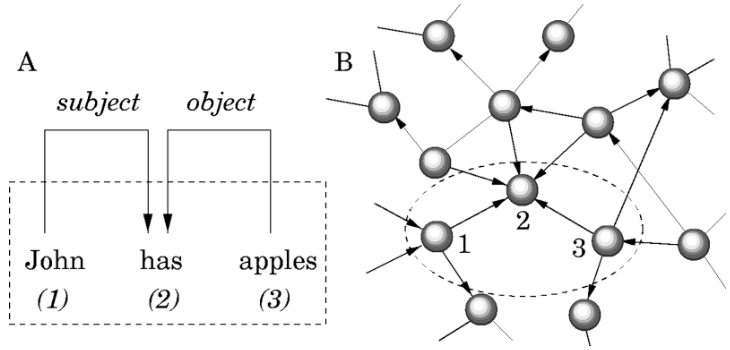
\includegraphics[width=0.5\textwidth]{figures/sdn.png}
    \caption{(a) The syntactic structure of a simple sentence. Here words define the nodes in a graph and the binary relations (arcs) represent syntactic dependencies. Here we assume arcs go from modifier to its head. The proper noun “John” and the verb “has” are syntactically dependent in the sentence. John is a modifier of the verb has, which is its head. Similarly, the action of has is modified by its object “apples.” (b) Mapping the syntactic dependency structure of the sentence in (a) into a global syntactic dependency network. Extracted from \cite{i2004patterns}}
    \label{fig:sdn}
\end{figure}